\begin{figure*}
  \begin{center}
    \begin{tabular}{c}
      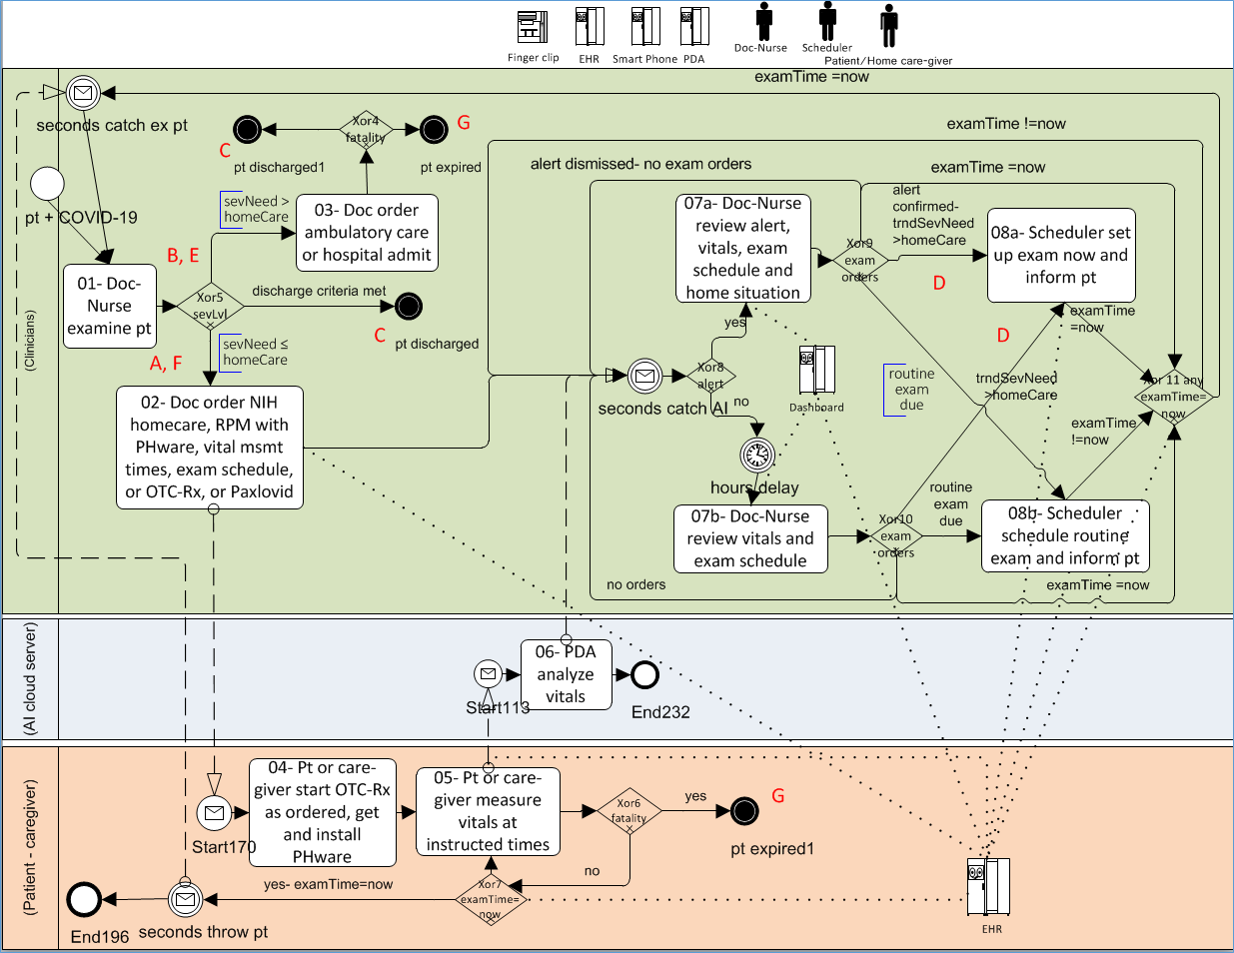
\includegraphics[width=6.98in]{bpmn.png}
    \end{tabular}
  \end{center}
\caption{The \href{https://github.com/ericmercer/SPIN-bpmn-cwp-verification-paper/blob/main/16-Feb-2022-BPMN-resources.png}{workflow model} for the \phware\ system.}
\label{fig:bpmn}
\end{figure*}

\figref{fig:bpmn} shows the PHware system design was developed in the \emph{Business Process Model Notation} (BPMN) \cite{BPMN} \cite{BPMNSpecification} using the The MATH tool-suite \cite{workflowmodel}.
The colored lanes represent the activities of clinicians, AI cloud services, and patient/care-givers.
The benefits of adapting BPMN to health care informatics are demonstrated by the recent \emph{BPM+} project of the Object Management Group.\footnote{Many thanks to Stephen White for reviewing the workflow and clarifying aspects of the BPMN semantics.}

Our method for functional integration was adapted from concurrent design engineering in aerospace, where specific tracks for multiple design disciplines coordinate their work by referencing a common physical design artifact \cite{10.1007/978-1-4471-1538-0_9}.
The technology-neutral CWP is pivotal for integrating cognitive work, and extends the notion of higher-order unification \cite{10.1007/3-540-45685-6_2} to joint, human-computer teaming. The CWP served as the common artifact for concurrent engineering, and the colored lanes as tracks to design the coordinated activity of clinicians, AI cloud services, and patient-caregivers. %to transform the CWP to establish and maintain \emph{actionable risk awareness}.

\figref{fig:bpmn} starts in the upper left of the green clinicians' workflow with postive test results that get exams in task-01. 
The bold letters in the text correlate to transitions of the CWP in \figref{fig:cwp}.
If exams find comorbidities, or moderate, or severe the flow goes to task-03 where the patients get ambulatory care or hospital admission (\textbf{B}/\textbf{E}).
Severity needs that can be met by home care flow to task-02 that orders home care (\textbf{A}/\textbf{F}).

The tan workflow of home care by patient/caregiver begins with task-04, then task-05 repeats recording vitals at ordered times until a new exam order loops back to task-01, or the patient expires (\textbf{G}). 
The exam can order more home care (back to task-04) or clinical care (task 03), or discharge (\textbf{C}.
Discharge requires a negative test following a recovery period.

The raw vitals data are transmitted by smartphone app to AI cloud services in the middle, metallic lane. The Personal Data Analyzer uses machine-learned algorithms in task-06 to assign numerical vital sign values to the sensor data, then analyzes the longitudinal trends of vital signs.
A packet of values and trends is sent immediately to the upper-right of the clinicians' green workflow. An elevated risk alert is added if any combination of current/trending values exceed home care capability.

Alerts skip any routine delay for clinicians' attention in task-07a. A specialized dashboard used in tasks-07a/b provides risk awareness of each patient.
The workflow and user interface were designed to preserve clinicians' ultimate decision authority.
They can quickly access AI reasoning, confirm the current/trending severity justifies the alert, or dismiss it.
If alerts are confirmed task-08a orders urgent teleheath exams that can be set up quickly with real-time vital signs.
Urgent exams may give orders for ambulatory care or hospital admission (\textbf{E}).

Clinicians may also decide trends can be controlled by adjusting orders for more frequent vitals, or oral medication for new discomfort, or \emph{Paxlovid}\textsuperscript{\texttrademark}\ to reduce progression. (\textbf{F}).
When multiple patients have alerts, providers must prioritize them based on familiarity and professional judgement.

If alerts are dismissed routine exams still may be ready to begin soon, or routine exams may be due for scheduling in task-08b. 
For non-alerts, providers review vitals in task 07b when time permits. They may order routine exams that are due to be scheduled by task 08b.
Alternatively, if clinical judgment deems appropriate, providers may order urgent exams in task 08a.
The far right decision gate \textbf{Xor11} is where all exam times are managed.
All approaching exams, whether urgent or scheduled, flow back to task-01, then are held when all participants arrive.